

%nicht kompletter Groebner fan

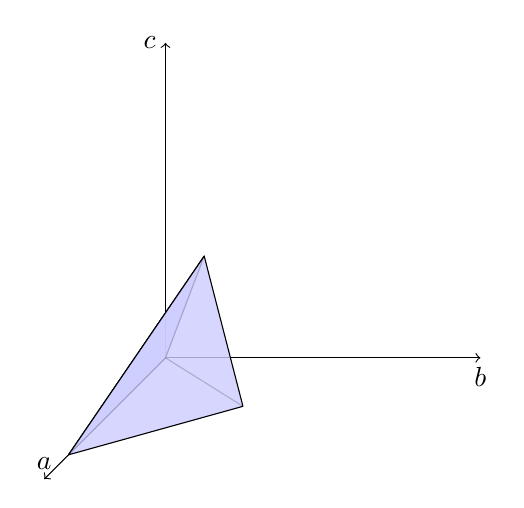
\begin{tikzpicture}[join=round,scale=0.8]
    \tikzstyle{conefill} = [fill=blue!20,fill opacity=0.8]
    \tikzstyle{ann} = [fill=white,font=\footnotesize,inner sep=1pt]
    \tikzstyle{ghostfill} = [fill=white]
    \tikzstyle{ghostdraw} = [draw=black!50]
    
    \draw[arrows=->,line width=.4pt](0,0,0)--(0,0,5); %Z_achse
    \draw[arrows=->,line width=.4pt](0,0,0)--(0,5,0); %Y-ACHSE
    \draw[arrows=->,line width=.4pt](0,0,0)--(5,0,0); %X-ACHSE
    %\draw[arrows=<-,line width=.4pt](.42,-.767)--(4,-2);
    
    \path (5,0,0) node[below] {$b$} (0,0,5) node[above] {$a$} (0,5,0) node[left] {$c$};
    
% letzte Koordinate ist A!!!
% zweite Koordinate ist C!!!
% dritte Koordinate ist B!!!
  
\filldraw[conefill](0,0,0)--(0,0,4)--(1,2,1)--cycle;
\filldraw[conefill](1,2,1)--(0,0,4)--(2,0,2)--cycle;
%\filldraw[conefill](1,2,1)--(0,0,0)--(2,0,2)--cycle;

\draw [opacity=0.2] (0,0,0) -- (2,0,2) ;
 
   
\end{tikzpicture}